\subsection*{The Phase 2 2La result}

Across nine populations, expected heterokaryotype frequency and suppression depth had Pearson \(r=\PhaseTwoPearsonR\) (\(P=\PhaseTwoPearsonP\)) and Spearman \(r_s=\PhaseTwoSpearmanR\) (\(P=\PhaseTwoSpearmanP\)). Both positive estimates were imprecise and neither test rejected the null. The heat map and statistics use the same checksum-bound maps; smoothing is confined to display and does not alter the 100-kb values used for inference.

\subsection*{A second LD estimator provides local corroboration}

Across three representative Phase 2 cohorts, mean matched-subsample rank concordance between \fastrho and pyrho was \PhaseTwoPyrhoMeanR{} on 3R:6--14 Mb (Fig.~\ref{fig:phase2-pyrho}). Both estimators use the same haplotypes and can share LD-related biases; agreement therefore supports estimator reproducibility, not contemporary crossover accuracy.

\begin{figure}[!htbp]
\centering
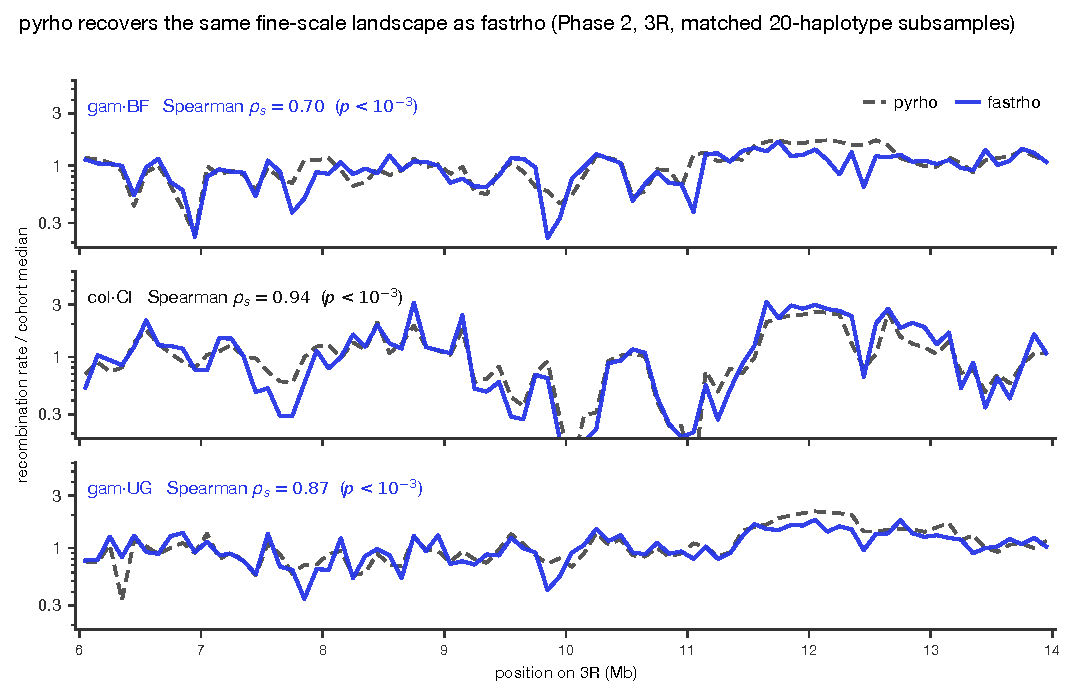
\includegraphics[width=0.82\textwidth]{figures/fig_phase2_pyrho.pdf}
\caption{\textbf{Local pyrho corroboration of selected Phase 2 map segments.} Solid cobalt \fastrho and dashed gray pyrho profiles use matched 20-haplotype subsamples from \texttt{gamb\_BF}, \texttt{colu\_CI}, and \texttt{gamb\_UG} along chromosome arm 3R (6--14 Mb), summarized in 100-kb windows and divided by each cohort's median. Annotations give two-sided Spearman correlations across windows.}
\label{fig:phase2-pyrho}
\end{figure}

\subsection*{The released crosses test broad spatial variation}

The caller retained \PhaseTwoCrossoverCount{} breakpoint intervals no wider than 1 Mb from \PhaseTwoProgenyCount{} progeny. Across \PhaseTwoPedigreeWindowCount{} supported 5-Mb windows, direct and atlas maps had Spearman \(r_s=\PhaseTwoPedigreeR\) (\(P=\PhaseTwoPedigreeP\)). The comparison uses all 11 crosses and the released SHAPEIT representation. It does not provide a held-out-family endpoint, genotype-quality sensitivity, absolute-rate calibration, or a test of individual resistance loci.

\subsection*{Resistance-panel result in Phase 2}

Across the nine populations, the median focal-to-haplotype-matched-control ratio for the 15 resistance regions was \PhaseTwoResistanceRatio{}. \PhaseTwoResistanceSignificantCount{} population-level permutation summaries were nominally below 0.05. Species-stratified median ratios were \PhaseTwoGambiaeResistanceRatio{} in \Agambiae and \PhaseTwoColuzziiResistanceRatio{} in \Acoluzzii. Despite variation among regions and cohorts, resistance-associated regions had lower inferred recombination overall, although this reduction was not observed at every region.
